% Section 6 - MDSplus
% Roberto Masocco <roberto.masocco@uniroma2.it>
% Alessandro Tenaglia <alessandro.tenaglia@uniroma2.it>
% June 5, 2024

% ### MDSplus ###
\section{MDSplus}
\graphicspath{{figs/section6/}}

% --- MDSplus ---
\begin{frame}{MDSplus}
	\begin{columns}
		\column{.6\textwidth}
		\textbg{MDSplus} is a tool for \textbg{data acquisition and storage}.\\
    \medskip
		\textbg{MDSplus} stores data in a user-defined hierarchical structure, namely a \textbg{tree}.\\
    \medskip
		A \textbg{tree} is formed by \textbg{nodes}, each of which represents a \textbg{data field}.\\
    \medskip
		Experiments of the same type have the same tree structure and an \textbg{incremental pulse number}.\\
    \medskip
    Trees contents can be inspected with:
    \begin{itemize}
      \item \textbg{jScope} to plot signals;
      \item \textbg{jTraverser} to navigate the tree, inspect nodes and their values;
      \item \textbg{MDSReader}, \textbg{MDSWriter} DataSources.
    \end{itemize}
		\column{.4\textwidth}
		\begin{figure}
			\centering
			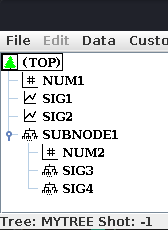
\includegraphics[scale=.5]{tree.png}
			\caption{Example of MDSplus tree\\visualized with jTraverser.}
			\label{fig:tree}
		\end{figure}
	\end{columns}
\end{frame}
